\documentclass{article}
\usepackage[usenames,dvips]{color}
\usepackage[utf8]{inputenc}
\usepackage{amsmath}
\usepackage{graphicx}
\usepackage[top=1.55cm, bottom=2.29cm, left=1.6cm, right=1.47cm]{geometry}
\usepackage{fancyhdr}
\usepackage{hyperref}
\hypersetup{
  colorlinks   = true, %Colours links instead of ugly boxes
%  urlcolor     = \color{MidnightBlue}, %Colour for external hyperlinks
%  linkcolor    = \color{MidnightBlue}, %Colour of internal links
%  citecolor   = \color{MidnightBlue} %Colour of citations
}

\lhead{}
\chead{}
\rhead{Implementación de Space Invaders en FPGA}
\pagestyle{fancy}
% Spanish support:
\usepackage[utf8]{inputenc}
%\usepackage[T1]{fontenc}
\usepackage[spanish]{babel}



% Initial pararagraph blankspace
\makeatletter 
\renewcommand{\paragraph}{\@startsection{paragraph}{4}{\z@}{-3.25ex \@plus 
-1ex \@minus -.2ex}{1.5ex \@plus .2ex}{\normalfont\normalsize\bfseries}} 
\makeatother

% Makes figures stay in place:
\usepackage{float}

\usepackage{parskip}
\setlength{\parindent}{15pt}

\begin{document}

%%%% FRONTPAGE %%%%%%%%%%%%%%%%%%%%%%%%%%%%%%%%%%%%%%%%%%%%%%%%%%%%%%%%%%%
\begin{center}

\includegraphics[width=0.25\textwidth]{./uc3m.jpg}\\[2cm]
\textsc{\LARGE Universidad Carlos III de Madrid}\\[0.5cm]
\textsc{\Large Diseño de Circuitos Digitales}\\[4cm]


% Title
{\huge \bfseries{Implementación de Space Invaders en FPGA}\\[8cm]}


% Author and supervisor
\begin{minipage}{0.55\textwidth}
\begin{flushleft} \large
\emph{Autores:}\\
David Estévez Fernández\\
Sergio Vilches Expósito\\
\end{flushleft}
\end{minipage}
\begin{minipage}{0.4\textwidth}
\begin{flushright} \large
\emph{Profesora:}\\
Anna Vaskova
\end{flushright}\end{minipage}\vfill

% Bottom of the page
{\large \today}

\end{center}
%
\newpage
%
%%%%%%Table of contents%%%%%%%%%%%%%%%%%%%%%%%%%%%%%%
%%%%%%%%%%%%%%%%%%%%%%%%%%%%%%%%%%%%%%%%%%%%%%%%%%%%%
\tableofcontents
\newpage

% Adds a newline after each paragraph
%\addtolength{\parskip}{\baselineskip}
%\setlength{\parskip}{0.3cm plus4mm minus3mm}

\section{Introducción}
\label{introduction}

El objetivo de esta práctica de laboratorio era realizar un diseño e implementación de un circuito digital con un juego inspirado en el arcade clásico ``Space Invaders'', en el lenguaje de descripción de hardware VHDL.

\begin{figure}[H]
	\centering
	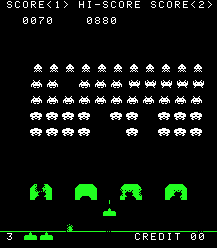
\includegraphics[width=0.4\textwidth]{SpaceInvaders-Gameplay.png}
	\caption{Pantalla del juego ``Space Invaders'' original }\label{fig:originalInvaders}
\end{figure}

Este juego, que ha sido simplificado para la consecución de este laboratorio, consiste en una nave, controlada por el jugador y localizada en la parte inferior de la pantalla, que se enfrenta a una serie de ``Invasores del espacio'', que van descendiendo por la pantalla. El jugador gana si elimina a todos los invasores, y pierde si los invasores llegan a la parte inferior de la pantalla, invadiendo la Tierra.

Para su implementación hardware se dispone de una placa entrenadora Spartar 3E Starter Board, la cual posee una FPGA Spartan 3E (modelo xc3s500E-4 FG320 ) así como distintos periféricos, como LEDs, pulsadores, interruptores, un encoder, conector VGA, etc. Para nuestra implementación hemos utilizado algunos de estos periféricos, como los LEDs, el conector VGA y 2 interruptores, así como un pin de salida, al que hemos conectado un jack de audio con un filtro paso bajo, para los sonidos y dos de los conectores de expansión de la placa, a los que hemos conectado unos mandos diseñados y construidos por nuestros compañeros del año pasado, Ruy García y Nieves Cubo, que nos los han prestado amablemente.

\newpage
\section{Funcionamiento general}
\label{generalBehavior}

El sistema final se muestra en la figura \ref{fig:spaceinvblock}. El sistema cuenta con los bloques básicos requeridos por el enunciado de la práctica, así como una serie de bloques extra añadidos como mejora del diseño básico. Estos bloques se explicarán de forma detallada en la sección \ref{blocksexplanation}, junto a las razones tras su implementación y cómo se llevaron a cabo las pruebas de los distintos bloques.

\begin{figure}[H]
	\centering
	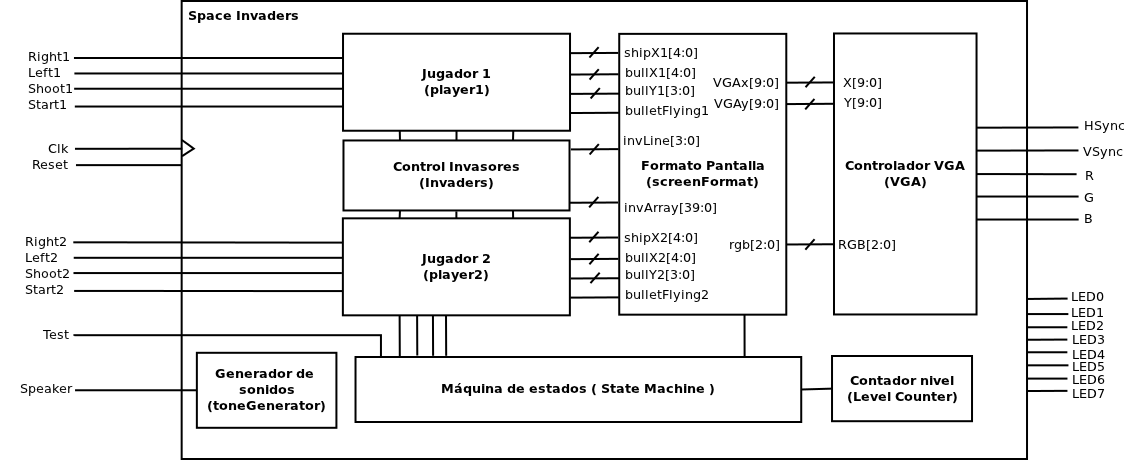
\includegraphics[width=\textwidth]{spaceinvaders.png}
	\caption{Diagrama de bloques del sistema completo. Algunas conexiones no se han indicado por claridad. }\label{fig:spaceinvblock}
\end{figure}

Los bloques básicos incluyen:
\begin{itemize}
	\item {\bfseries Controlador VGA}: Encargado de generar la señal de control de la pantalla.
	\item {\bfseries Formato Pantalla}: Su función es dibujar los distintos elementos del juego en su correspondiente posición de la pantalla.
	\item {\bfseries Control Invasores}: Controla el movimiento de los marcianos y su desaparición tras un disparo.
	\item {\bfseries Control nave}: Controla el movimiento de la nave del jugador.
	\item {\bfseries Control disparo}: Controla el movimiento del disparo.
	\item {\bfseries Detector de flancos}: Convierte la señal de entrada de los pulsadores en un pulso apto para el circuito.
	\item {\bfseries Máquina de estados}: Controla el flujo del juego.
\end{itemize}

Además de esos bloques, se han implementado como mejora los siguientes:
\begin{itemize}
	\item {\bfseries Jugador}: Agrupa varios elementos del jugador, como la nave, el disparo y los detectores de flancos, además de contar la puntuación de ese jugador. Es de gran utilidad para incluir dos jugadores en el juego.
	\item {\bfseries Sintetizador de sonidos}: Genera sonidos de estilo \textit{arcade} que acompañan diferentes acciones del juego.
	\item {\bfseries Contador de nivel}: sirve para seleccionar la velocidad de juego y dificultad de los marcianos dependiendo de las pantallas ganadas.
	\item {\bfseries Otros}: Además de los bloques anteriores, se han modificado algunos de los bloques básicos para extender su funcionalidad.
\end{itemize}

El mecanismo del juego es el siguiente. Al accionar el interruptor de test en cualquiera de los estados se mostrará en la pantalla un patrón de prueba (tablero de ajedrez) y la partida se reiniciará. El juego se inicia en el estado inicial, en el que se muestra la pantalla de juego estática. En este estado inicial un segundo jugador puede activar la señal de inicio para sumarse a la partida, de forma que pueden jugar 1 ó 2 jugadores. Al pulsar el botón de inicio el jugador 1 el juego se inicia, los invasores comienzan su movimiento y los jugadores pueden moverse y disparar una bala cada vez. 

Si los invasores alcanzan el final de la pantalla, la partida se termina y los jugadores pierden. Si, por el contrario, los jugadores consiguen alcanzar a todos los invasores, superan la pantalla y el nivel se incrementa en 1, pudiendo jugar el siguiente nivel hasta un máximo de 8 niveles, en los que la dificultad de los marcianos y la velocidad de los mismos aumenta. Existen 3 tipos de invasores, verdes, amarillos y blancos, que requieren 1, 2 y 3 disparos respectivamente para morir. Cada disparo acertado aumenta la puntuación de ese jugador en 1 unidad. Si se pierde la partida en cualquiera de los niveles los jugadores deben empezar de nuevo desde el primer nivel (no se dispone de vidas extra).

\newpage

\section{Explicación de los bloques}
\label{blocksexplanation}
%
\subsection{Controlador de pantalla VGA}
\label{vga}

\begin{figure}[H]
	\centering
	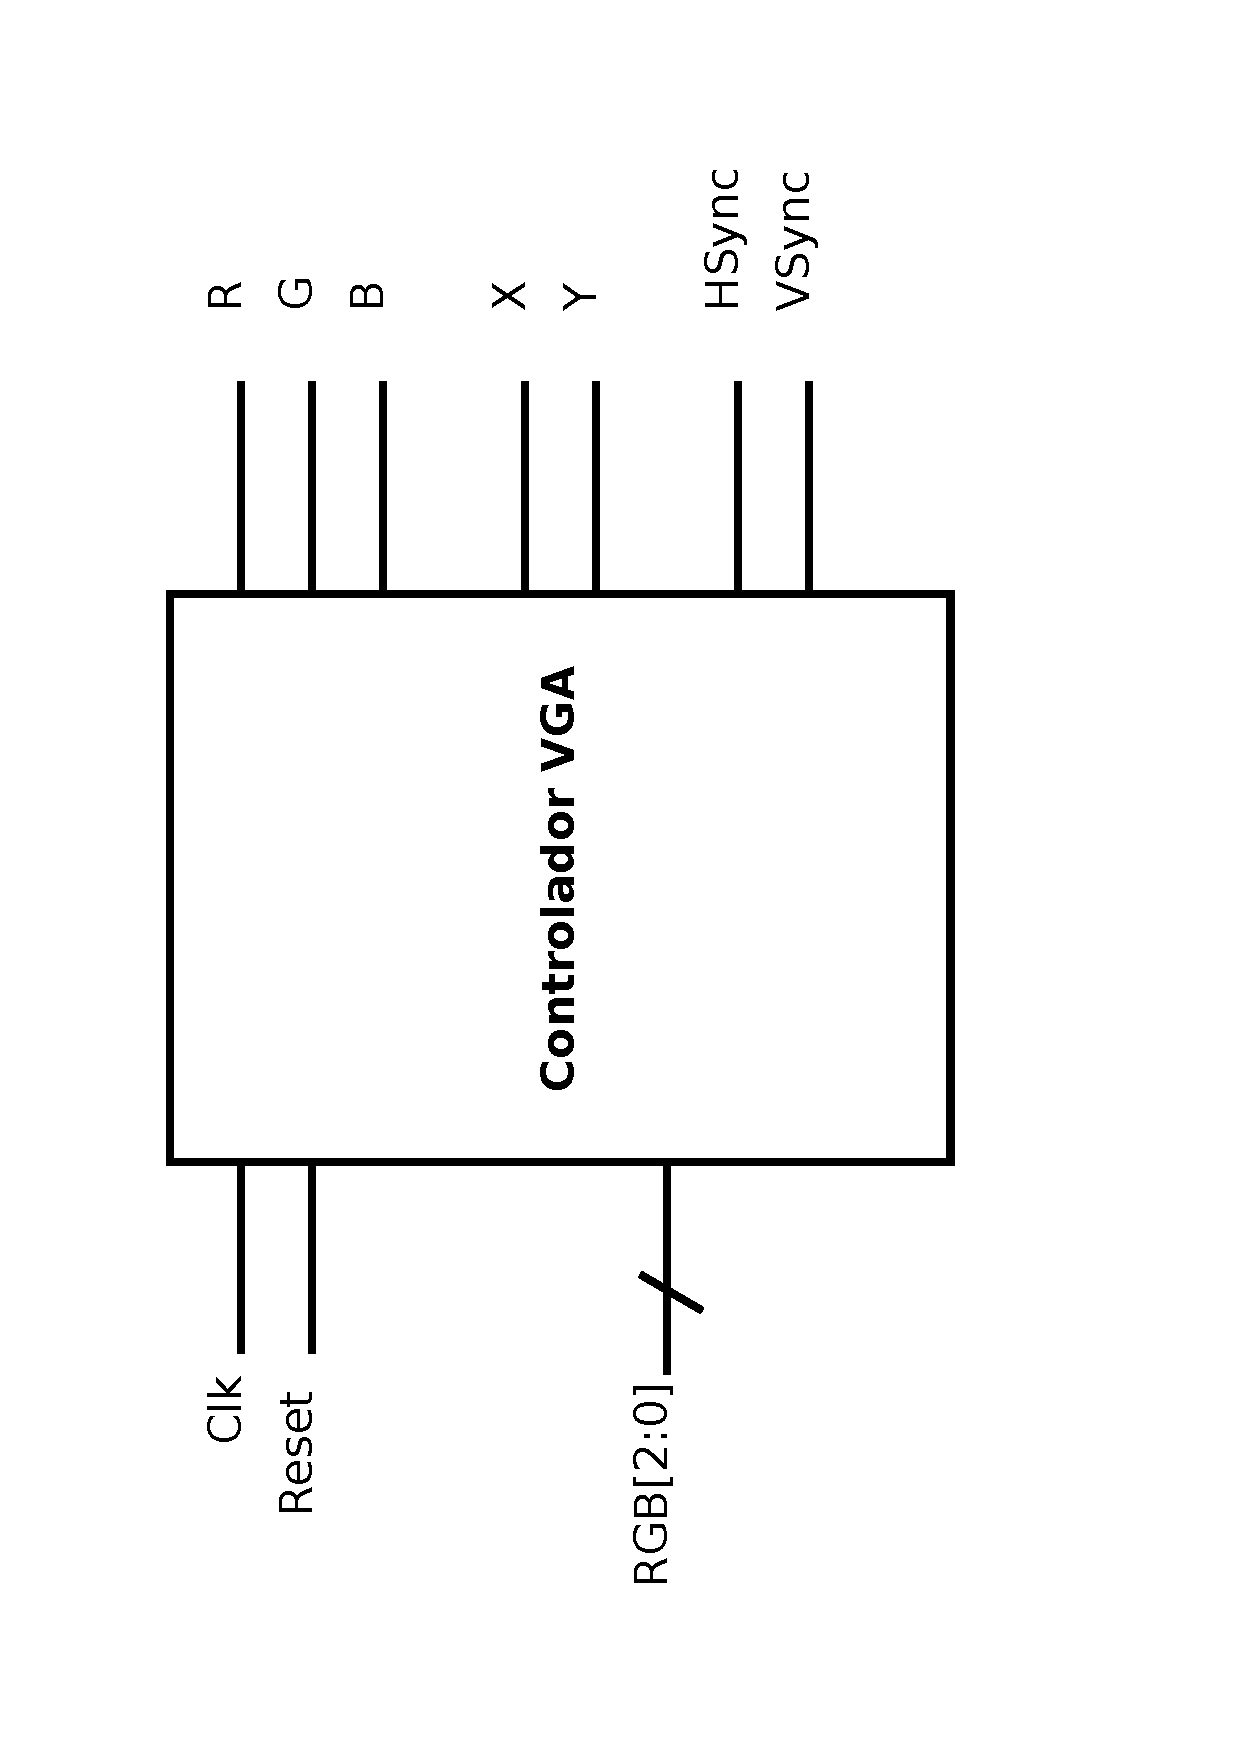
\includegraphics[width=0.4\textwidth, angle=-90] {vga_block.pdf}
	\caption{Interfaz del controlador de pantalla VGA}\label{fig:vgaBlock}
\end{figure}

El controlador de pantalla VGA se encarga de generar el patrón de ondas necesario para mostrar los gráficos del juego en una pantalla externa.

\subsubsection{Descripción Funcional}

El estándar VGA usa tres señales analógicas para codificar el color de cada píxel (R, G y B en la figura \ref{fig:vgaBlock}) y dos señales de sincronización que indican el fin de línea $HSync$ y fin de pantalla $VSync$). Para la implementación del controlador se ha usado una frecuencia de 25 MHz, que genera una resolución de 640 x 480 píxeles a una tasa de refresco de 60 Hz.

Para formar la imagen deseada en la pantalla, el controlador VGA accede a la información de color de cada píxel de manera similar a una memoria: las señales x e y indican la posición del píxel al bloque \hyperref[formatoVGA]{Formato VGA}, que devuelve el valor del color a través del bus $RGB$. 

Dado que la placa de desarrollo \emph{Spartan 3E Starter Kit} contiene un conversor digital a analógico (DAC) de un sólo bit para las señales $R$,$G$ y $B$, sólo es posible mostrar 8 colores diferentes en la pantalla.

\subsubsection{Implementación}

Las señales VGA \textit{HSync} y \textit{VSync} son siempre periódicas y están controladas por dos contadores en cascada: \textit{HCount} (con valores de 0 a 800) y \textit{Vcount} (0 a 521). El contador horizontal \textit{HCount} proporciona un marco temporal para mostrar los 640 píxeles que hay en cada línea de la pantalla, terminando cada ciclo con pulso bajo en \textit{HSync}, indicando que el monitor debe comenzar una nueva linea. 

Cada vez que se termina una línea, el contador vertical \textit{VCount} aumenta su valor hasta completar una pantalla (480 líneas). Entonces, un pulso bajo en \textit{VSync} indica al monitor que debe comenzar una nueva imagen.

Estos contadores usan un \emph{prescaler} de 1 bit, ya que la señal \textit{clk} tiene una frecuencia de 50 MHz pero la interfaz con la pantalla está configurada a 25 MHz.



\subsection{Formato VGA}
\label{formatoVGA}

\begin{figure}[H]
	\centering
	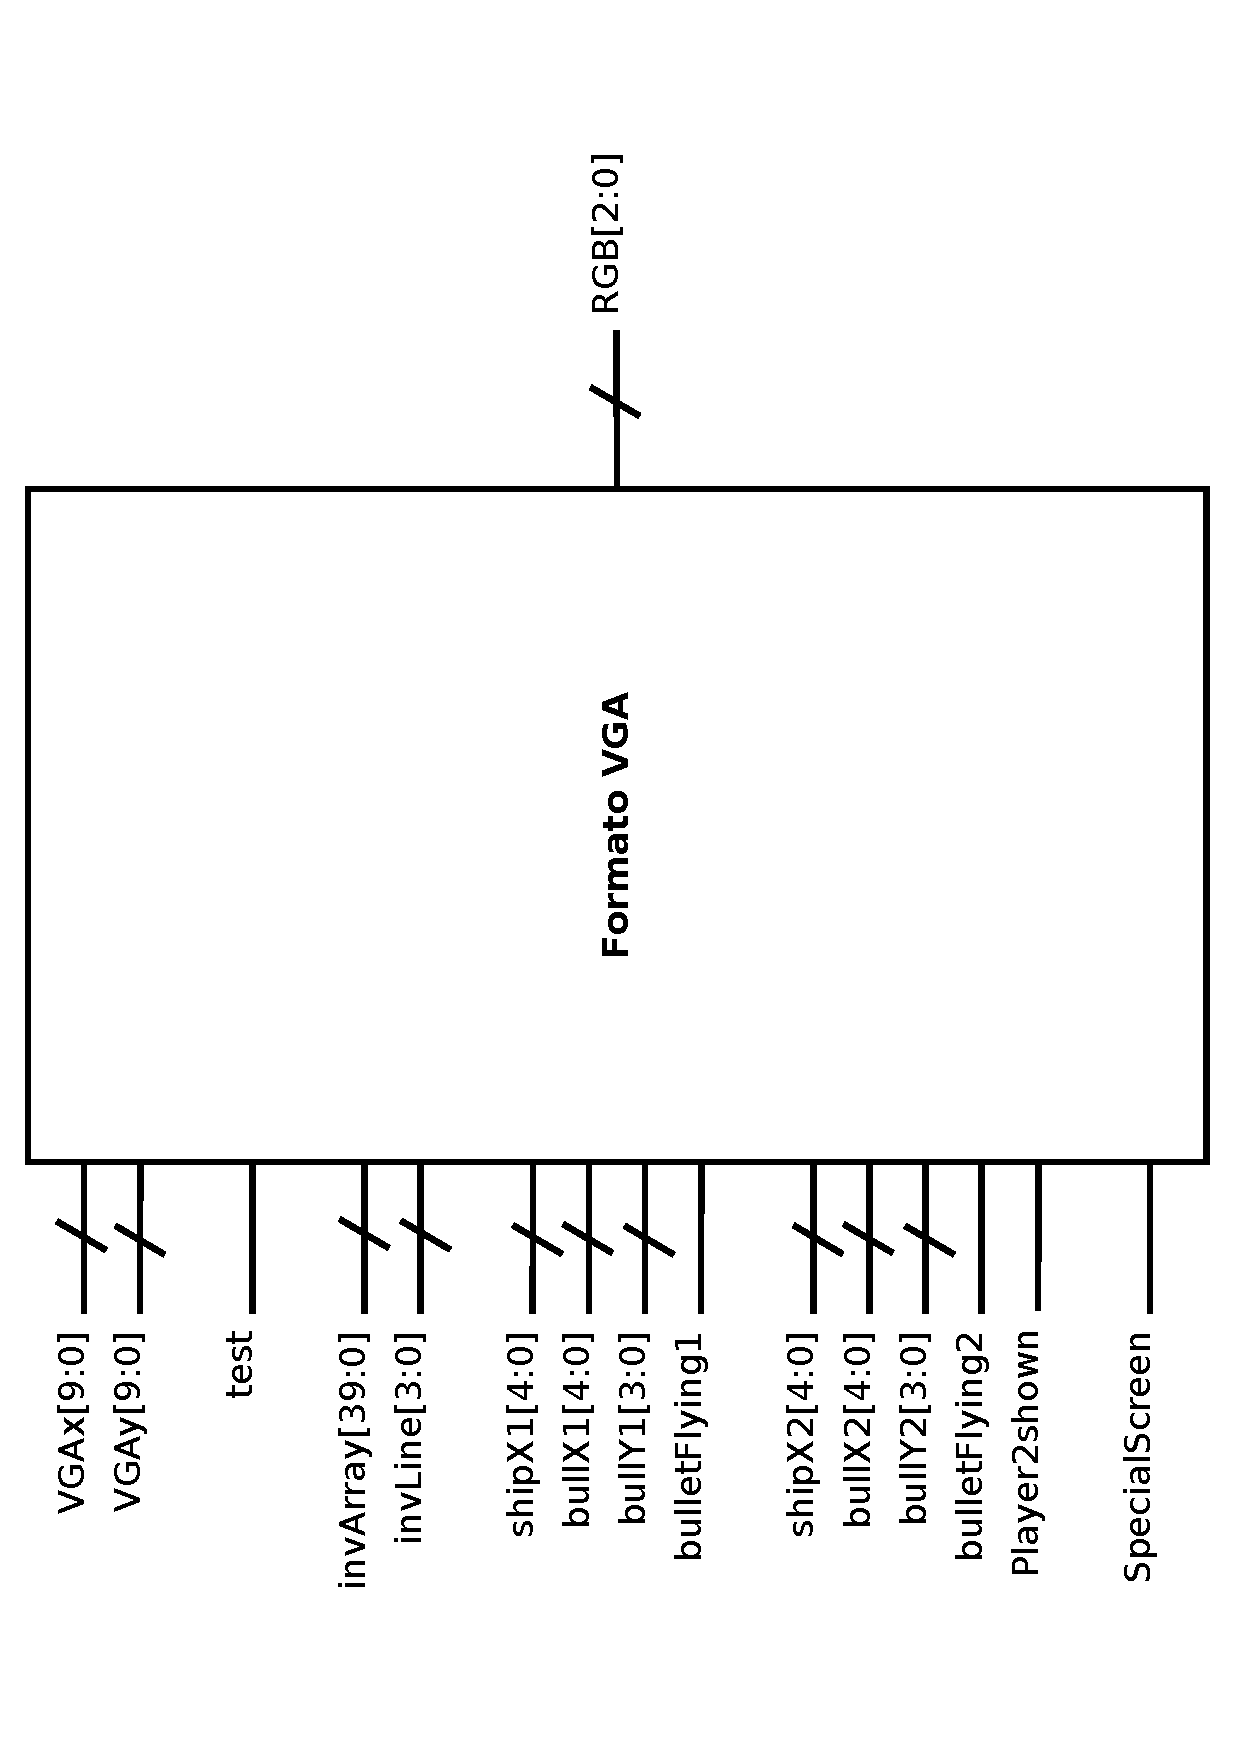
\includegraphics[width=0.4\textwidth, angle=-90] {formatoVGA_block.pdf}
	\caption{Interfaz del bloque Formato VGA}\label{fig:formatoVGA_block}
\end{figure}





El bloque \emph{Formato VGA} se encarga de traducir una serie de señales binarias procedentes de los invasores, naves y balas a figuras (\emph{sprites}) que mostrar en la pantalla.

\subsubsection*{Descripción del proceso}

Para facilitar esta tarea, la pantalla se divide en \emph{macropíxels}, celdas de 32 x 32 píxeles que contienen un sólo sprite. Así, el espacio de juego queda reducido a una matriz de 20 x 15 macropíxels. 

El proceso de dibujo de la pantalla pude resumirse de la siguiente manera:

\begin{enumerate}

\item El controlador VGA solicita la información RGB de un píxel.

\item \emph{Formato VGA} traduce la posición (x,y) a su correspodiente macropíxel.

\item Con la información procedente del resto de entidades, se selecciona qué elemento hay que mostrar en ese macropíxel.

\item Se accede a la matriz del sprite correspondiente, obteniedo el valor del píxel en concreto que se ha de dibujar.
\end{enumerate}

\subsubsection*{Codificación de la posición de los elementos}

La información posicional de los invasores, balas y naves se envía desde los diversos bloques a través de buses, que codifican la información de manera diferente:

\begin{itemize}
\item \textbf{Bala}: Cada una de las dos balas transmiten su posición en coordenadas de macropíxels, codificadas en dos buses de 5 y 4 bits respectivamente ($bullX_n$, $bullY_n$). La señal $bulletFlying_n$ indica si la bala de cada uno de los jugadores está activa.

\item \textbf{Nave:} Como la nave sólo puede moverse en la última línea de la pantalla, la señal $shipX_n$ basta para indicar su posición en el juego. Adicionalmente, la señal $player2shown$ indica si hay que mostrar la nave del jugador 2.

\item \textbf{Invasores:} La posición de cada uno de los invasores, así como su tipo, se codifica en las señales $invLine$ y $invArray$. $invLine$ define en qué linea se mueven los invasores, mientras que $invArray$ codifica el estado de los invasores (activo o abatido) y su nivel (más información en \hyperref[invaders]{Invasores}).

\end{itemize}
\subsection{Detectores de flancos}
\label{edgeDetectors}

Para la interfase del diseño con los pulsadores diseñamos dos detectores de flancos, uno estándar y otro antirrebotes, de forma que llegase un sólo pulso a los demás bloques del sistema por cada pulsación del jugador.

En el diseño final sólo hemos añadido el detector de flancos con antirrebote, debido a su mejor respuesta ante la entrada oscilante de los pulsadores reales.

\subsubsection{Detector de flancos estándar (edgeDetector)}
\label{edgeDetectorStd}
El detector de flancos estándar es un circuito muy simple. Se tienen dos biestables, uno almacenando el estado actual de la señal de entrada, y el otro almacenando el estado de la señal en el tiempo t-1.

Estas dos señales se comparan, y si hay un nivel alto en el estado actual, pero no en el anterior, entonces ha llegado un flanco, y el detector emite un pulso a la salida.

\paragraph{Banco de pruebas}
En el banco de pruebas de este bloque se simuló una entrada de una duración superior a 1 periodo de reloj, con la señal de habilitación (``Enable'') activada y desactivada, de forma que se comprobó que la salida al llegar un flanco con el enable activado era de un pulso exacto.

\subsubsection{Detector de flancos con antirrebote (edgeDetectorDebounce)}
\label{edgeDetectorDebounce}

\begin{figure}[H]
	\centering
	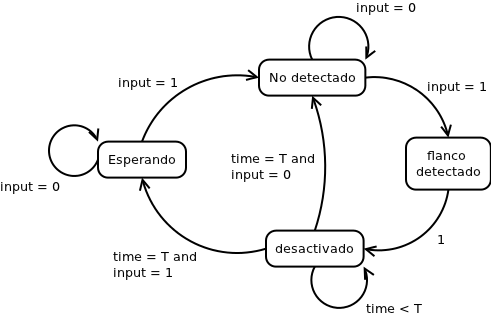
\includegraphics[width=0.5\textwidth]{edgeDetectorDebounceFSM.png}
	\caption{Máquina de estados}\label{fig:edgeDetectorDebounceFSM}
\end{figure}

El detector de flancos con antirrebote es un detector de flancos estándar al que se le ha añadido un temporizador que lo desactiva durante un cierto periodo de tiempo tras detectar un flanco, para evitar las oscilaciones producidas por los rebotes de los pulsadores.

Su diseño está basado en una máquina de estados simple (figura \ref{fig:edgeDetectorDebounceFSM}) que consta de cuatro estados: ``no detectado'', ``flanco detectado'', ``desactivado'' y ``esperando''. La máquina empieza en el estado ``no detectado'', y permanece en él mientras la entrada valga 0. Cuando recibe un 1, pasa al estado ``flanco detectado'', y la salida se pone a 1 hasta el siguiente flanco de reloj, en el cual pasa al estado
``desactivado'', poniendo la salida a 0. Mientras la máquina se encuentra en este estado, un temporizador cuenta el tiempo transcurrido, y bloquea el paso al estado siguiente. Cuando el tiempo deseado, en nuestro caso 100 ms,  ha transcurrido, la máquina de estados pasará al estado ``no detectado'' si la entrada es 0 o a ``esperando' si es 1. La máquina pasará entonces al estado de ``no detectado'' cuando reciba un 0 lógico.

\paragraph{Banco de pruebas}
Para probar este bloque se diseñó un banco de pruebas que simulaba una entrada ruidosa, con varias oscilaciones entre nivel alto y bajo, de forma que se comprobase que el detector sólo se activaba una vez tras el flanco, con una duración de un periodo de reloj.
\subsection{Máquina de estados principal}
\label{statemachine}

\begin{figure}[H]
	\centering
	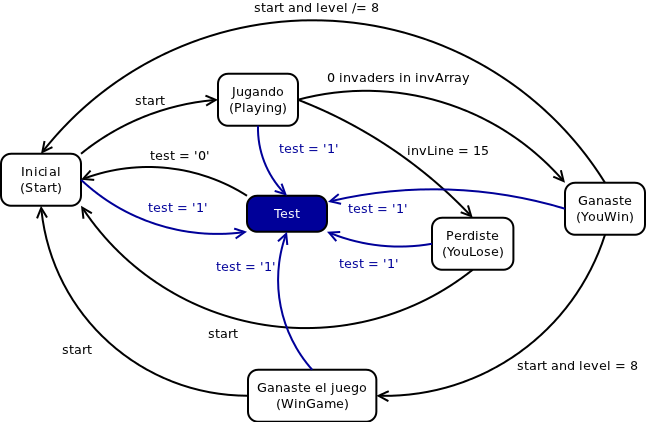
\includegraphics[width=0.6\textwidth]{statemachine.png}
	\caption{Diagrama de estados }\label{fig:statemachine}
\end{figure}

El control del flujo del juego y el funcionamiento de los distintos bloques se lleva a cabo con una máquina de estados. Algunas señales, cuya lógica de activación es más compleja, se activan a partir de las señales de estado en un proceso independiente, que se explicará a continuación. La máquina de estados posee los siguientes estados:

\begin{itemize}
	\item {\bfseries Test}: estado de prueba. Se llega a él desde cualquier estado tras activarse la señal ``test'' y cuando la máquina está en este estado se reinician todos los valores de la partida y se muestra en la pantalla un patrón de tablero de ajedrez.
	\item {\bfseries Inicial (Start)}: en este estado la máquina está esperando que el jugador inicie la partida. Los bloques de ambos jugadores se reincian (excepto las puntuaciones) y desactivan, y el bloque de los invasores se reinicia y permanece parado. Al recibir una señal de inicio ( ``p1StartPulse'') del jugador 1, se pasa al estado ``jugando (playing)''.	
	\item {\bfseries Jugando (Playing)}: este estado corresponde al juego propiamente dicho. En él se inicia el movimiento de los invasores y se habilitan los controles de los jugadores. Desde este estado se pasará a ``ganaste (YouWin)'' si se han eliminado todos los invasores y el vector ``invArray'' sólo contiene `0's, o a ``perdiste (YouLose)'' si los invasores consiguen llegar al final de la pantalla, es decir, si invLine = 15.
	\item {\bfseries Perdiste (YouLose)}: este estado muestra la pantalla de juego perdido. Se permanece en este estado mientras no se reciba una señal de inicio ( ``pxStartPulse'') de cualquiera de los dos jugadores (que lleva la máquina al estado inicial), y en él los invasores y los jugadores permanecen reiniciados y deshabilitados.
	\item {\bfseries Ganaste (YouWin)}: este estado se muestra la pantalla de juego ganado. Se permanece en este estado mientras no se reciba una señal de inicio ( ``pxStartPulse'') de cualquiera de los dos jugadores (que lleva la máquina al estado inicial siempre y cuando no se halla superado el último nivel), y en él los invasores y los jugadores permanecen reiniciados y deshabilitados. Al llegar a este estado se habilita una señal que hace que el contador de nivel se incremente una unidad, haciendo que al volver al estado inicial los invasores que aparezcan sean de una dificultad superior.
	\item {\bfseries Ganaste el Juego (WinGame)}: se llega a este estado tras haber finalizado el último nivel, y en él se muestra la pantalla de juego completado. Este estado reinicia tanto los invasores como los jugadores, y se queda a la espera de una señal de inicio ( ``pxStartPulse'') de cualquiera de los dos jugadores para iniciar una nueva partida.
\end{itemize}

Además de las señales que se controlan de forma combinacional dentro de la máquina de estados, se han añadido algunas señales dependientes del estado o de la transición, cuya lógica de activación es ligeramente más compleja, en procesos independientes. 
Más concretamente, se ha añadido un biestable que contiene la señal de activación del jugador 2, que se acciona cuando nos encontramos en la pantalla de inicio de nivel (``Start'') y recibimos una señal de inicio del jugador 2 (``p2StartPulse), y se reinicia al perder la partida o ganar el juego (una vez el jugador 2 se une a la partida, permanece habilitado hasta que la partida acaba). También se ha añadido un proceso que reinicia las puntuaciones y el nivel cuando se produce una transición desde un estado que no sea ``Ganaste (YouWin)'' hasta el estado ``Inicial (Start)''.
\subsection{Jugador (Player)}
\label{player}

\begin{figure}[H]
	\centering
	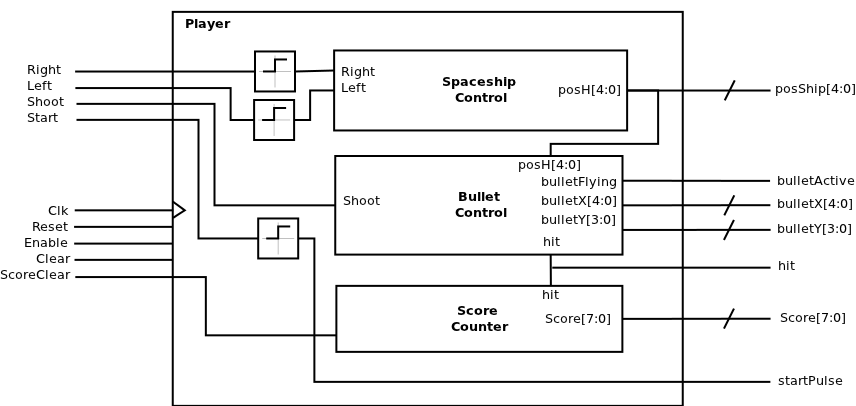
\includegraphics[width=0.6\textwidth]{player_block.png}
	\caption{Diagrama de bloques del Jugador (player) }\label{fig:playerBlock}
\end{figure}

Con el fin de agrupar todas las funciones de un jugador para mayor claridad, hemos creado un bloque Jugador (Player) que incluye toda la funcionalidad del jugador, de forma que además podemos instanciar varios jugadores de forma sencilla. Esto ha facilitado el añadir un segundo jugador a nuestro juego, simplemente instanciando este bloque 2 veces.

El bloque Jugador (figura \ref{fig:playerBlock}) incluye: tres detectores de flancos con antirrebote para las señales de movimiento a izquierda y derecha y de inicio, un control de la nave, un control del disparo y un contador para la puntuación.

También posee una serie de señales de control del bloque: Reset asíncrono, Clear síncrono ( pone todo a su estado inicial excepto la puntuación), un Clear síncrono para la puntuación y una entrada Enable para su habilitación, que afecta a todos los bloques excepto al detector de flancos de inicio, que siempre está activo.

La implementación en VHDL simplemente instancia los bloques necesarios y realiza las conexiones entre ellos. El contador de la puntación, sin embargo, se ha implementado como un proceso, que incrementa una unidad el contador cada vez que le llega una señal de marciano alcanzado por un disparo (hit).


\subsection{Control de los invasores (Invaders)}
\label{invaders}

\begin{figure}[H]
	\centering
	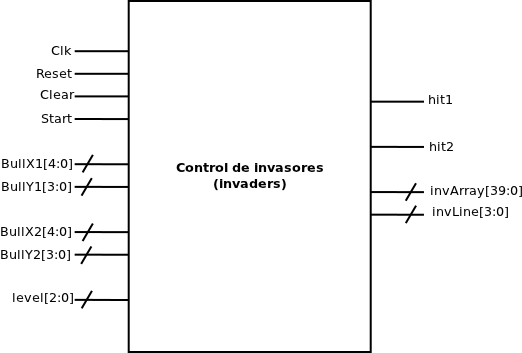
\includegraphics[width=0.4\textwidth]{invaders_block.png}
	\caption{Diagrama de bloques del Control de los invasores (Invaders) }\label{fig:invadersBlock}
\end{figure}

El bloque de control de los invasores se encarga tanto del movimiento de los invasores a lo largo de la pantalla, como de comprobar la posición del disparo y matar a los correspondientes marcianos. Para ello, además de las entradas de control típicas (Clk, Reset, Clear) posee 2 conjuntos de entradas que le proporcionan la posición y estado de cada una de las 2 balas del juego (una por cada jugador).

Para ello hemos definido una matriz constante que almacena la disposición inicial de los marcianos para cada uno de los 8 niveles implementados. Esta disposición se selecciona a través de la entrada ``level'', que indica el nivel actual.

Existen tres tipos de invasor, dependiendo del número de vidas que tengan (verde, 1 vida; amarillo, 2 vidas y blanco, 3 vidas) que se codifican usando 2 bits, siendo 00 un hueco sin marciano, 01 un marciano verde, 10 un marciano amarillo y 11 un marciano blanco, de 3 vidas. Estos marcianos se guardan en un vector de 40 elementos, 2 elementos por casilla de la pantalla en la que puede haber un marciano, que como se ha mencionado previamente, se selecciona dependiendo del nivel actual.

Este bloque también posee dos temporizadores que controlan la velocidad de avance de los invasores. Dependiendo del nivel se selecciona uno u otro, teniendo dos velocidades posibles (normal y rápida). Se seleccionó este diseño en lugar de un sólo temporizador con 8 velocidades (una por nivel) debido a que al haber aumentado la dificultad añadiendo marcianos más poderosos no tenía mucho sentido incrementarla aún más aumentando la velocidad en sólo 8 niveles, y había recursos suficientes en la FPGA como para poner dos teporizadores, cuyo diseño ya estaba realizado en prácticas anteriores, en lugar de uno nuevo con varias comprobaciones de cuenta.

La implementación en VHDL posee una señal ``start'', que sirve de señal de disparo, cambiando el estado de un biestable interno ``moving'' que indica al bloque que los marcianos han comenzado a moverse. Una vez en movimiento, cada pulso de reloj (en el que el temporizador lo permita), el vector de marcianos sufre un desplazamiento de 2 posiciones hacia la derecha. Si una de las 2 últimas posiciones del vector contiene un 1, es decir, si un marciano ha llegado al final de la línea, la posición en el eje Y se incrementa una unidad, y se invierte el sentido del desplazamiento. Este proceso se repite hasta que todos los marcianos hayan muerto, o hayan llegado a la última posición.

Por último se comprueba si el disparo coincide con la posición de alguno de los marcianos, y si es así, decrementa la vida del marciano en 1 unidad (un marciano blanco pasaría a ser amarillo, uno amarillo a ser verde, y uno verde moriría) y envía un pulso a través de la señal ``hit1'' o ``hit2'', dependiendo de qué jugador haya alcanzado al marciano.
\newpage
\section{Conclusión / Posibles mejoras}
%
\end{document}